\chapter{Análisis limitaciones actuales}

\incomment{Antes de esto se deben haber explicado las arquitecturas de 
referencia WR, si no hacerlo aquí.}

El proyecto \gls{wr} ofrece dos tipos de arquitectura como referencia: la 
orientada a dispositivos que actúen como \gls{bc}, y la enfocada a nodos 
finales \gls{oc}. En la sección \ref{sec:wr} \incomment{esto no es verdad aún} 
se ha visto que para la primera se cuenta 
con un dispositivo de referencia, el \gls{wrs}, que implementa la arquitectura 
de \gls{bc} y en la cual se centra el desarrollo \textit{oficial}. La segunda 
se materializa en la tarjeta \gls{spec} como ejemplo básico de nodo \gls{wr}.

La línea de desarrollo seguida desde la empresa Seven Solutions y desde el 
grupo de investigación enfocado en \gls{wr} de la UGR se ha centrado en el 
desarrollo de las arquitecturas de referencia y en el diseño de nuevos tipos de 
arquitecturas que solucionen las deficiencias presentes en los diseños 
iniciales.

\incomment{con ese comentario quiero dejar claro que parte del trabajo 
mencionado corresponde a otras personas pero de forma sutil}

Aunque la estrategía no es la misma si se habla de la arquitectura de 
\textit{switch} que si se hace de la de nodo, si es cierto que hay una 
corriente que se comparte en ambos desarrollos: la utilización de los nuevos 
modelos de \gls{soc} para lograr un mayor nivel de integración y un aumento de 
las prestaciones del sistema sin elevar la complejidad del mismo en exceso.

En el caso del \gls{wrs} existente se han detectado varios problemas por la 
gran complejidad del diseño \textit{hardware} que tiene el circuito 
electrónico. 
Uno de ellos es la comunicación entre el procesador ARM y el circuito  
implementado en la lógica reconfigurable de la \gls{fpga}. Gracias a la mejora 
en la 
tecnología de fabricación se consiguen actualmente sistemas que integran tanto 
\gls{fpga} como microprocesador en un único chip reduciendo costes y 
complejidad de desarrollo.

La arquitectura referencia para los nodos \gls{wr} ha tratado de ofrecer un 
diseño básico y asequible económicamente. El uso de la familia Spartan de 
Xilinx ha permitido mantener los costes bajos a la vez que ha permitido alojar 
el diseño básico de la arquitectura de nodo \gls{wr} . Sin embargo, dicho 
diseño se está mejorando y está recibiendo cada vez más funcionalidades por lo 
que la necesidad de recursos está creciendo. Además, dicho diseño tiene una 
limitación bastante importante: carece de un microprocesador dedicado lo que 
dificulta en gran medida el desarrollo e incorporación de nuevas 
características. De igual forma que en la arquitectura de \textit{wrs} se 
tiende hacía soluciones en \gls{soc}, la arquitectura de nodo se puede 
beneficiar de este tipo de soluciones ya que permiten incluir un 
microprocesador físico en el diseño sin necesidad de gastar puertas para 
incluirlo y además mantener los costes bajos.

Mi trabajo de investigación se ha enfocado en la arquitectura de nodo por lo 
que será a la que haga referencia en el resto de la memoria, aunque como he 
comentado en los párrafos anteriores, muchas de las mejoras planteadas a 
continuación se pueden incorporar en la arquitectura tipo \textit{switch}.

\incomment{contextualizar lo siguiente}
El primer paso para poder plantear mejoras a la arquitectura de nodo y al 
rendimiento de la sincronización en los mismos es establecer el punto de 
partida. Para ello se ha realizado una labor de análisis de una arquitectura 
actual de nodo basada en un diseño similar al de la tarjeta \textit{spec} pero 
que ya presenta una serie de mejoras.

El nodo utilizado como punto de partida es el WR-LEN \cite{website:len}
desarrollado por Seven Solutions. Dicho dispositivo incorpora una versión 
mejorada del \gls{wrc} denominado \gls{wrc2p} cuya principal característica es 
la inclusión de un segundo puerto físico a la arquitectura de nodo.

\subsection{White Rabbit Core Dual Port}

El \gls{wrc2p} \cite{felipe16} es una extensión de la arquitectura para nodos 
\gls{wr} 
denominada \acrlong{wrc} \incomment{refs} que añade una segunda interfaz física 
Ethernet a la arquitectura básica mono-puerto. En la implementación actual, la 
referencia temporal es única para ambos puertos, lo que supone que el 
dispositivo puede actuar como nodo (esclavo o maestro) y como \gls{bc}, es 
decir, esclavo de un nivel superior de la jerarquía de red y maestro de un 
nivel inferior. Además, se pretenden desarrollar técnicas que habiliten la 
redundancia (hacer un cambio de referencia si un enlace se cae). 
\incomment{mejorar la redacción de eso.}

Esta nueva arquitectura de nodo extendida permite el desarrollo de dispositivos 
\gls{bc} de coste reducido que son ideales para su uso en topologías lineales, 
donde el uso de \gls{wrs}s supone una infrautilización de los puertos 
disponibles por equipo.

\begin{figure}
	\centering
	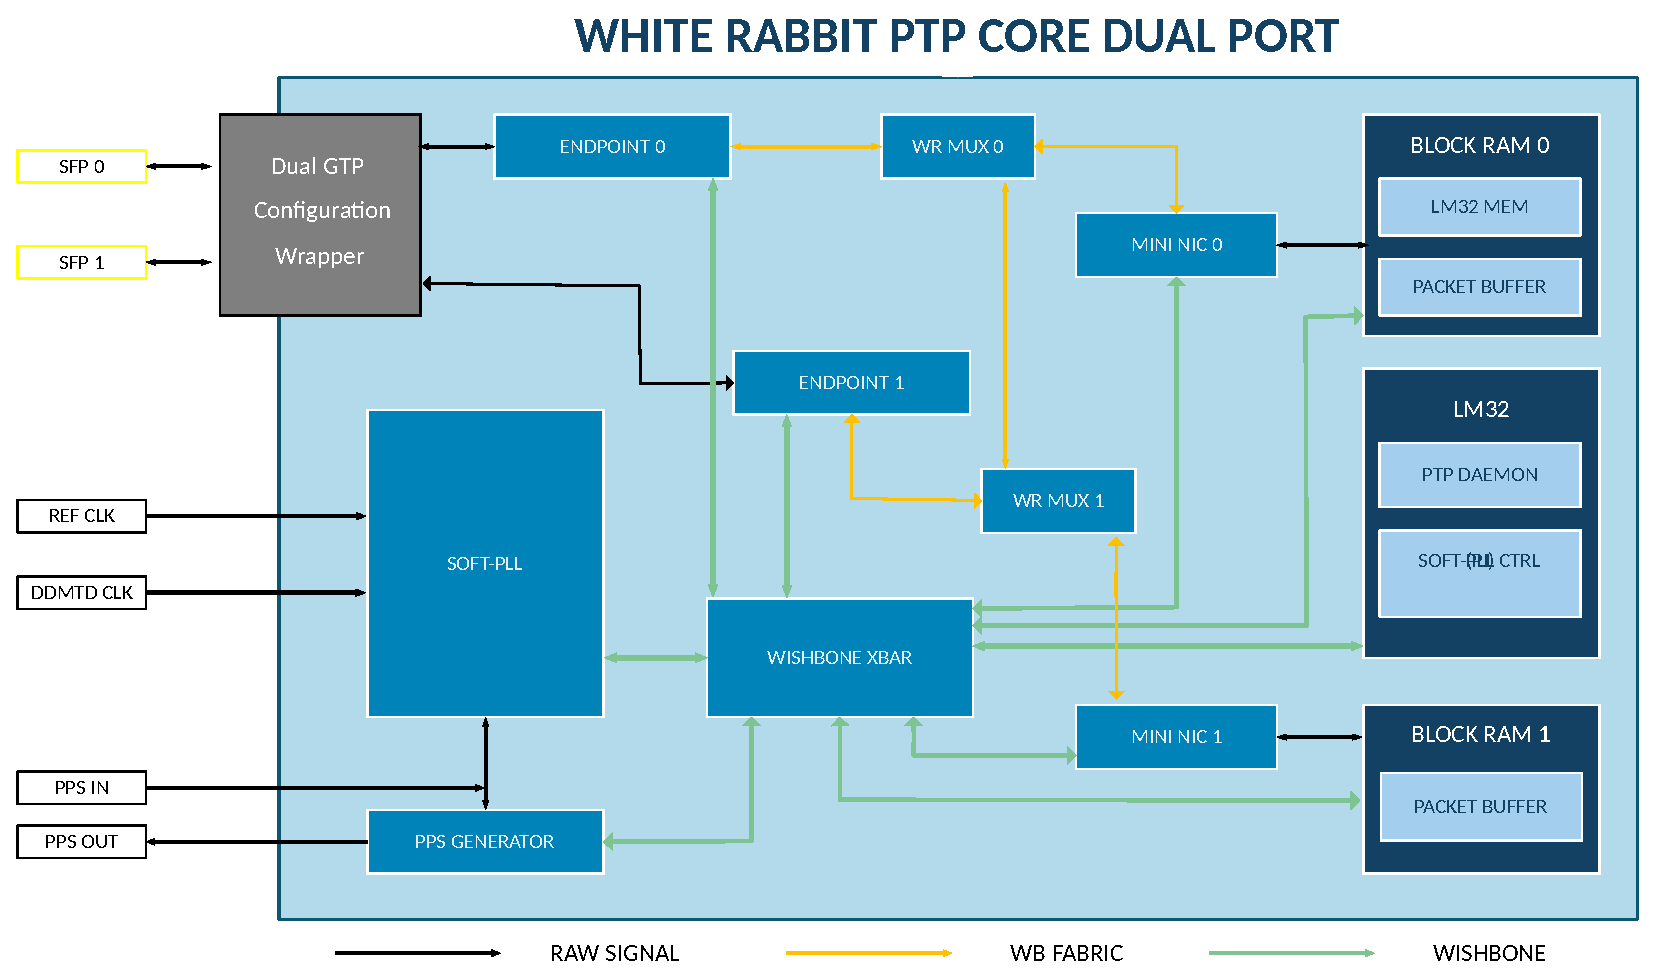
\includegraphics[width=0.7\linewidth]{imagenes/wrpc_dp}
	\caption[Diagrama de bloques del WRC2P]{Este diagrama muestra la estructura 
	de módulos HDL para el diseño de la arquitectura WRC2P.}
	\label{fig:wrpcdp}
\end{figure}


La Figura \ref{fig:wrpcdp} muestra como se organizan los módulos para la 
arquitectura de \gls{fpga}. Con respecto al diseño de referencia se realiza una 
duplicación de los componentes principales de la lógica de \gls{wr}: 
\textit{endpoint}, multiplexor WR, mini-NIC
y los módulos de RAM. Sin embargo el bloque para el procesador embebido se 
mantiene, realizando únicamente cambios a nivel de \textit{sw}. Con ello se 
consigue reducir el número de puertas necesarias, algo clave para alojar la 
arquitectura dentro de una FPGA de perfil bajo.

\subsection{WR-LEN}

El WR-LEN es el primer dispositivo \gls{wr} en incorporar la arquitectura 
\gls{wrc2p}. Fue diseñado por la empresa Seven Solutions y está disponible 
desde 2015. Sus principales características son la inclusión de un segundo 
puerto físico compatible con \gls{wr}, conectores coaxiales de tipo \gls{sma} y 
una tercera interfaz Ethernet de tipo 1000BaseT.

\begin{figure}
	\centering
	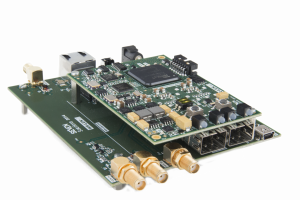
\includegraphics[width=0.7\linewidth]{imagenes/wrlen}
	\caption[WR-LEN en su versión para desarrolladores]{Imagen de un equipo 
	WR-LEN sin caja. Se puede observar como se compone de dos tarjetas: la 
	principal (arriba) donde se sitúa la electrónica de control de WR, y el 
	\textit{backplane} (abajo) que dota de interfaces de entrada/salida a la 
	primera.}
	\label{fig:wrlen}
\end{figure}


La electrónica encargada de la recuperación de reloj y mantenimiento de la 
referencia de tiempo local se mantiene con respecto a la utilizada en el 
\gls{wrs}. \incomment{si antes no se ha hablado del wrs elec. hablar aquí} El 
único cambio reseñable se encuentra en el reloj utilizado para los módulos 
\gls{ddmtd} que ya no utiliza un \gls{pll} externo para generar la frecuencia 
de 62.5 MHz necesaria, si no que se aprovecha uno de los \gls{pll} internos de 
la \gls{fpga} para ello. \incomment{que hice con los resultados?}

\incomment{debería decir algo más de la electrónica, es cerrado así que tampoco 
quiero pasarme...}

\subsection{Experimentos de escalabilidad}

Para evaluar las limitaciones del \gls{wrc2p} en cuanto a prestaciones y 
escalabilidad realicé una serie de experimentos encadenando múltiples nodos 
\gls{wr}. A través del análisis de la señal de reloj de salida producida por 
la lógica de \gls{wr} se pueden obtener indicadores de como de estable es el 
proceso de sincronización en cada nodo, o dicho de otra forma, cuanto ruido 
electromagnético se añade a la señal fundamental de \gls{wr} por cada salto. La 
hipótesis de partida es que debido al ruido electromagnético y demás fuentes 
posibles de inestabilidad debe de existir un número máximo de nodos 
sincronizables bajo las condiciones de exactitud de WR, es decir, en algún 
momento se perderá el sub-nanosegundo. Además, si el aumento del nivel de ruido 
es alto, llegará un momento en el que ni siquiera sea posible sincronizar, 
debido a que la frecuencia recuperada del enlace esté fuera de rango para el 
bucle de control que disciplina el oscilador del nodo. Para comprobar dichas 
hipótesis se han propuesto una serie de experimentos cuyos resultados deben 
permitir establecer los límites de la implementación 
(comprobar si se cumple la exactitud sub-nanosegundo) y detectar las 
deficiencias o mejoras posibles a fin de mejorar el diseño existente.

\begin{figure}
	\centering
	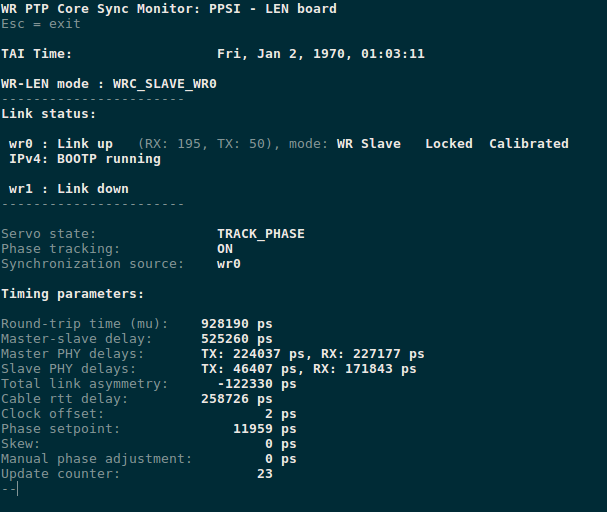
\includegraphics[width=0.7\linewidth]{imagenes/len_gui}
	\caption[Captura del monitor WR en el dispositivo WR-LEN]{Esta captura 
	muestra la información que aporta el monitor interactivo WR para el caso de 
	un nodo. Los datos más importantes son los relativos a la hora del sistema, 
	el modo de operación y el estado del servo. Además se ofrecen estadísticas 
	del enlace como el \textit{round-trip time} o la asimetría.}
	\label{fig:lengui}
\end{figure}


De las alternativas disponibles en el universo de los dispositivos WR, se ha 
utilizado la arquitectura basada en nodo, y en concreto 
WR-LENs para realizar este tipo de pruebas: por un lado, los resultados 
obtenidos se pueden extrapolar a otros diseños como el del \gls{wrs}. Esto se 
debe a que el mecanismo de sincronización es prácticamente el mismo en ambas 
arquitecturas. Y por el otro, está el sentido práctico: realizar una cadena de 
muchos equipos es complejo en cuanto a la gran necesidad de material y recursos 
en el laboratorio. El uso de equipos simples como el WR-LEN ha hecho posible 
llegar a conectar un elevado número de nodos en cascada (hasta 18) permitiendo 
así observar el comportamiento de la tecnología en una red con un gran número 
de saltos (o \textit{hops}).

El primer experimento está pensado para comprobar si efectivamente la 
sincronización se deteriora hasta el punto de no lograr sincronizar un equipo 
(aunque sea fuera del nanosegundo de diferencia).
Para ello se desplegó una red de WR-LEN conectadas en cadena, tal como muestra 
la Figura \ref{fig:chainschema}. Para comprobar la exactitud de la 
sincronización en los puntos elegidos, se toma el reloj de salida del nodo 
maestro como referencia y el reloj del nodo esclavo i-ésimo, y con la ayuda de 
un osciloscopio de alta resolución se toman muestras de la diferencia en el 
dominio del tiempo entre los flancos de subida de las señales de reloj o de los 
PPSs.

\incomment{hablar del proc. de calibración (o mejor en la parte de ruido como 
en retos?) y decir que se ha calibrado aquí.}

Para comprobar si un nodo logra sincronizarse, además de observar las señales 
de salida, se debe consultar el monitor de estado de \textit{wr}. En la Figura 
\ref{fig:lengui} se incluye una captura de dicho monitor. \incomment{explicar 
el contenido del monitor si hay ganas} Como se ha mencionando anteriormente, 
este primero experimento busca 
determinar en que momento un nodo es incapaz de sincronizarse con el resto de 
la red. Para determinarlo, se debe ir conectando uno a uno cada dispositivo y 
comprobar el estado de la sincronización es \textit{Track-Phase}. 
Además se puede ir comprobando que la diferencia en tiempo entre las señales de 
\gls{pps} del maestro \textit{free-running} y de cada nodo sea inferior al 
nanosegundo. Las pruebas se han tomado por período de una hora y cada 
experimento se ha repetido tres veces para comprobar la consistencia de los 
resultados.

\begin{figure}
	\centering
	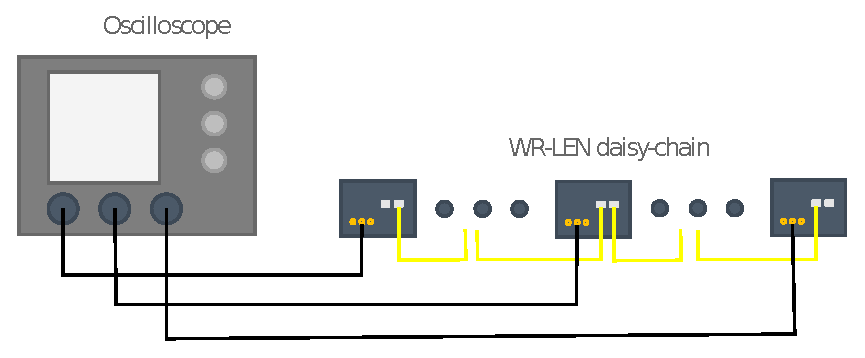
\includegraphics[width=0.7\linewidth]{imagenes/chain_schema}
	\caption[Esquema de conexión para los experimentos de escalabilidad.]{El 
	esquema muestra como se han conectado los diferentes nodos que han 
	compuesto la red WR para los experimentos de escalabilidad. Cada nodo actúa 
	como esclavo del nivel inferior y como maestro del siguiente (cascada).}
	\label{fig:chainschema}
\end{figure}

\begin{table}
	% increase table row spacing, adjust to taste
	\renewcommand{\arraystretch}{1.3}
	% if using array.sty, it might be a good idea to tweak the value of
	% \extrarowheight as needed to properly center the text within the cells
	\caption{Medidas de desfase para el primer experimento de la cascada de 
	WR-LEN con 18 nodos.}
	\label{tab:cascada1}
	\centering
	% Some packages, such as MDW tools, offer better commands for making tables
	% than the plain LaTeX2e tabular which is used here.
	\begin{tabular}{|c||c||c||c|}
		\hline
		Desfase & Mean & $\sigma$ & peak-to-peak \\
		\hline
		Maestro al 10º nodo & -212.51 ps & 45.653 ps & 312.50 ps \\
		\hline
		Maestro al 15º nodo & -500.66 ps & 174.50 ps & 1.0731 ns \\
		\hline
		Maestro al 18º nodo & -573.45 ps & 490.17 ps & 2.6487 ns \\
		\hline
	\end{tabular}
\end{table}

En el contexto de este análisis los valores más relevantes extraídos son los 
correspondientes a la desviación típica y al llamado \textit{peak-to-peak} que 
no es más que la diferencia entre el valor máximo y el mínimo. Con el primero 
nos podemos hacer una idea del ruido presente en el sistema y con el segundo se 
comprueba cuando, en el peor de los casos, la sincronización pierde en algún 
momento el nanosegundo de exactitud. ¿Por qué no interesa el valor medio? Al 
principio de la sección se ha mencionado que se han utilizado los mismos 
parámetros de calibración para todos los nodos \incomment{esto no es cierto 
aún}. Esto es algo típico y que 
funciona bastante bien cuando nos encontramos dentro de un escenario usual de 
red. Sin embargo, es totalmente posible realizar una calibración por nodo 
consiguiendo así que el valor medio esté centrado en 0. Dado que el foco de 
este análisis es el ruido y sus consecuencias, no se ha considerado relevante 
invertir tiempo en realizar un proceso de calibración completo que habría 
supuesto invertir mucho tiempo.

Los resultados numéricos de este primer experimento se incluyen en la Tabla 
\ref{tab:cascada1} y también se puede observar la distribución que siguen las 
muestras tomadas en la Figura \ref{fig:histexp1}. Se incluyen únicamente los 
resultados en los nodos 10º, 15º y 18º por motivos de reproducibilidad del 
experimento. Dado que el osciloscopio cuenta con 4 canales de entrada y uno de 
ellos es el utilizado por la referencia, solo se pueden tomar al mismo tiempo 
medidas de 3 nodos.
Del montaje inicial de la red se determinó que la sincronización 
sub-nanosegundo se consigue hasta el nodo 12º. Aunque los siguientes nodos se 
encuentran \textit{en media} dentro de rango, el análisis del peor de los casos 
muestra que es a partir del nodo 12º cuando no se puede asegurar que la 
diferencia entre la marca temporal del maestro y la del nodo sea siempre menor 
del ns \textit{explicar como se calcula eso que no es trivial}. Aún así los 
valores medios pueden ser interesantes para aplicaciones 
que no sean críticas y permitan cierta tolerancia a este fenómeno.
El otro resultado importante al que se llegó fue que a partir del nodo 18º no 
se consigue pasar de la fase de sintonización por lo que \gls{wr} no puede 
funcionar. Es decir, se comprobó que la hipótesis era cierta y el incremento 
del nivel de ruido por salto ocasiona un deterioro constante de la distribución 
de tiempo que llega hasta el punto de ser imposible sincronizar sin realizar 
ajustes en el algoritmo de control para relajar las condiciones del bucle de 
control.

Tras observar ambos resultados, se realizó una toma de medidas de desfase entre 
nodos clave: 10º, 15º y 18º. Los primeros nodos mostraban valores bajos de 
ruido por lo que resultaba más interesante analizar que pasaba cerca del punto 
donde se pierde la sincronización y al final de la cadena, donde el ruido 
comienza a ser muy elevado. Los resultados mostrados en la Tabla 
\ref{tab:cascada1} ayudan a comprender que falla para que a partir del nodo 18º 
no se consiga sintonizar. 

\incomment{hablar del pll, ancho de banda y relacionar con la teoría cuando 
esté}

Otro de las pruebas realizadas busca comprobar una de las hipótesis del procolo 
WWR de que la longitud 
del enlace de fibra óptica no tiene un efecto considerable sobra la precisión 
de la sincronización (siempre considerando una longitud dentro del rango de 
operación de los \gls{sfp}s utilizados). Para ello se replicó el montaje en 
cadena, pero utilizando menos nodos (15) pues los valores de los nodos finales 
en cadenas largas son muy inestables y aportan poca confianza estadística a la 
hora de determinar si hay diferencia o no entre usar un enlace corto o no. Las 
medidas de desfase se han tomado en los nodos 13º, 14º y 15º, usando un enlace 
de 5 km entre los nodos 13º y 14º.

\begin{table}
	% increase table row spacing, adjust to taste
	\renewcommand{\arraystretch}{1.3}
	% if using array.sty, it might be a good idea to tweak the value of
	% \extrarowheight as needed to properly center the text within the cells
	\caption{Medidas de desfase para el segundo experimento de la cascada de 
		WR-LEN usando fibras cortas.}
	\label{tab:cascada2}
	\centering
	\begin{tabular}{|c||c||c||c|}
		\hline
		Desfase & Mean & $\sigma$ & peak-to-peak \\
		\hline
		Maestro al 13º nodo & -368.82 ps & 117.08 ps & 694.23 ps \\
		\hline
		Maestro al 14º nodo & -367.75 ps & 173.45 ps & 971.43 ps \\
		\hline
		Maestro al 15º nodo & -766.19 ps & 235.77 ps & 1.373 ns \\
		\hline
	\end{tabular}
\end{table}

\begin{table}
	% increase table row spacing, adjust to taste
	\renewcommand{\arraystretch}{1.3}
	% if using array.sty, it might be a good idea to tweak the value of
	% \extrarowheight as needed to properly center the text within the cells
	\caption{Medidas de desfase para el segundo experimento de la cascada de 
		WR-LEN usando un enlace de 5 km entre los nodos 13º y 14º.}
	\label{tab:cascada3}
	\centering
	% Some packages, such as MDW tools, offer better commands for making tables
	% than the plain LaTeX2e tabular which is used here.
	\begin{tabular}{|c||c||c||c|}
		\hline
		Desfase & Mean & $\sigma$ & peak-to-peak \\
		\hline
		Maestro al 13º nodo & -341.08 ps & 101.02 ps & 507.05 ps \\
		\hline
		Maestro al 14º nodo & -271.06 ps & 234.52 ps & 859.52 ps \\
		\hline
		Maestro al 15º nodo & -700.65 ps & 203.93 ps & 1.5425 ns \\
		\hline
	\end{tabular}
\end{table}

Los resultados se incluyen en la Tabla \ref{tab:cascada2} para el caso de todos 
los enlaces con fibras cortas, y en la Tabla \ref{tab:cascada3} para el del 
enlace de varios kilómetros. Al igual que para el primer experimento se 
incluyen los histogramas de la distribución de las muestras en las Figuras 
\ref{fig:histexp2} y \ref{fig:histexp3} respectivamente. La diferencia 
observada entre los dos experimentos muestra que no hay diferencia 
significativa (los valores tienen una gran dispersión) entre el uso de un 
enlace de varios kilómetros o uno casi despreciable, tanto en el caso del nodo 
conectado con el enlace como en el siguiente. Además los resultados son 
consistentes con lo visto en el primero experimento: el nodo 13º se encuentra 
fuera (por poco) del ns en el peor de los casos, y el nodo 15º presenta una 
dispersión en torno a los 200 ps.

\begin{figure}
	\centering
	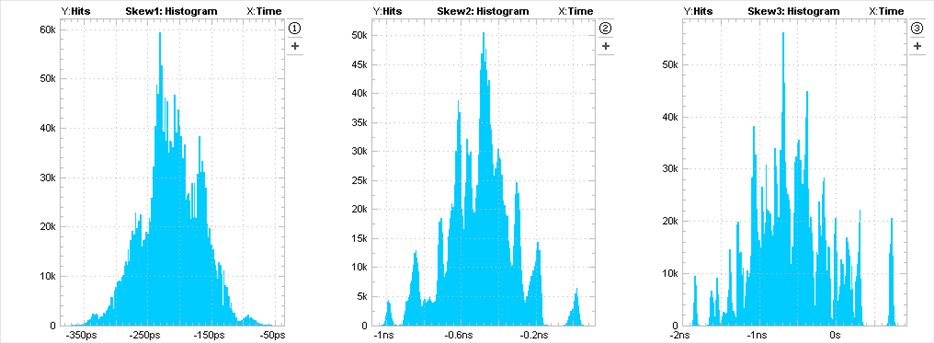
\includegraphics[width=0.7\linewidth]{imagenes/hist_exp1}
	\caption[Histograma para cadena de 18 WR-LEN]{Los histogramas muestran la 
	distribución de las muestras correspondientes a la diferencia entre las 
	señales de PPS en el maestro y la de los nodos 10, 15 y 18.}
	\label{fig:histexp1}
\end{figure}

\begin{figure}
	\centering
	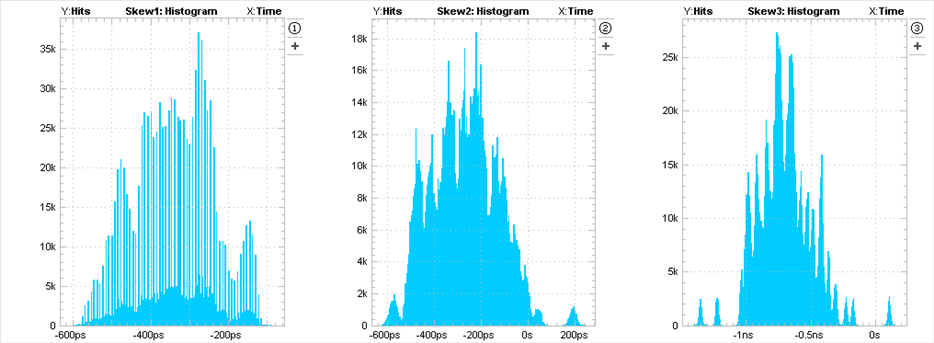
\includegraphics[width=0.7\linewidth]{imagenes/hist_exp3}
	\caption[Histograma para cadena de 15 WR-LEN]{Los histogramas muestran la 
		distribución de las muestras correspondientes a la diferencia entre las 
		señales de PPS en el maestro y la de los nodos 10, 15 y 18.}
	\label{fig:histexp2}
\end{figure}

\begin{figure}
	\centering
	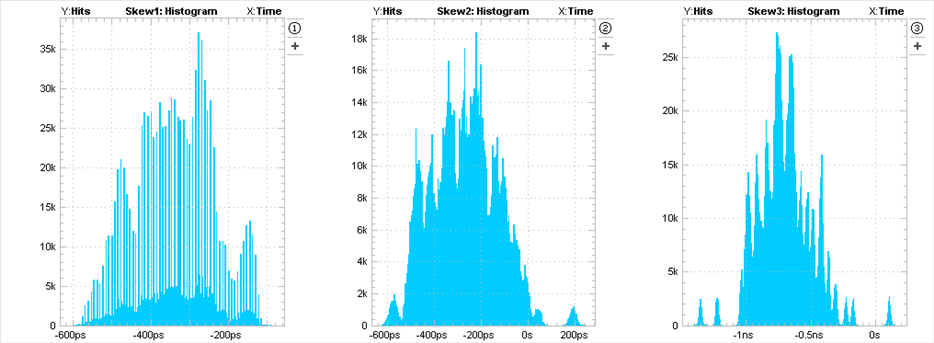
\includegraphics[width=0.7\linewidth]{imagenes/hist_exp3}
	\caption[Histograma para cadena de 15 WR-LEN con un enlace de 5km]{Los 
	histogramas muestran la distribución de las muestras correspondientes a la 
	diferencia entre las señales de PPS en el maestro y la de los nodos 10, 15 
	y 18.}
	\label{fig:histexp3}
\end{figure}

\subsubsection{Conclusiones}

Los experimentos realizados sobre una red de dispositivos \gls{wr} conectados 
en cascada han arrojado varios resultados interesantes y han permitido 
comprobar las hipótesis acerca del efecto del ruido en el sistema y us 
consecuencias:

\begin{itemize}
	\item Se ha realizado una caracterización de la implementación \gls{wrc2p}, 
	la cual extiende la funcionalidad de la arquitectura clásica de nodo 
	\gls{wr} manteniendo un diseño alojable en \gls{fpga}s de perfil bajo. Dado 
	que dicha implementación es relativamente nueva, era importante comprobar 
	que el nuevo diseño cumple las especificaciones básicas del protocolo  
	\gls{wr} antes de trabajar en las posibles mejoras.
	
	\item Se han obtenido resultados muy interesantes en cuanto a los límites 
	de la tecnología, observando que no se consiguen sincronizar más de 18 
	equipos en cadena. Este tipo de pruebas no se había realizado hasta la 
	fecha con un número tan elevado de equipos \gls{wr} por lo que dichos 
	resultados son de gran utilidad para el resto de la comunidad. Si bien los 
	resultados se han obtenido usando equipos de bajo perfil, la electrónica de 
	control es en su mayor parte idéntica a la usada por el \gls{wrs} por lo 
	que se puede extrapolar las conclusiones pensando que quizás en el caso de 
	una cadena de 18 \gls{wrs}s se podría obtener cierta mejora gracias a 
	contar con una \gls{fpga} de perfil alto que cuenta con ??gth en lugar 
	de ??gtp.
	
	\item Se ha comprobado la hipótesis de que gracias al nuevo modelo de 
	enlace presente en \gls{wr} se consigue calibrar de forma dinámica la 
	longitud del enlace de fibra óptica mediante la utilización del parámetro 
	de asimetría.
\end{itemize}

Además he podido comprobar de primera mano que aspectos son mejorables y la 
posible línea de trabajo futuro. En cuanto a la arquitectura de nodo, he 
detectado una serie de problemas que merece la pena discutir. En primer lugar, 
hay que entender ciertas decisiones del diseño inicial que se pudieron tomar 
para realizar un sistema que fuera sencillo y mantuviese los costes bajos. Con 
esto me refiero a la ausencia de un microprocesador físico externo que permita 
obtener un mayor rendimiento y flexibilidad de desarrollo para el \textit{sw} 
de la plataforma. El código \textit{sw} actual de un nodo se ejecuta en 
procesador embebido, el LM32. Este, cuenta con unos recuros muy limitados y se 
nota 
bastante a la hora de desarrollar para esta plataforma. Al incorporar una 
\gls{fpga} de perfil bajo, el número de recursos disponibles es limitado: hay 
pocas puertas lógicas disponibles y el número de bloques de memoria RAM es 
bajo. Eso provoca que el rendimiento de ejecución del LM32 sea bastante bajo y 
el desarrollo de nuevas características está limitado por la falta de recursos. 
Hay que tener en cuenta que este sistema se pensó en un primer momento para 
gestionar una única interrupción del \textit{Soft-PLL} y realizar el cálculo 
del desfase en tiempo real. Es el caso del \gls{wrs}, donde la única función 
del LM32 es esa. En el desarrollo de la arquitectura de nodo, al carecer de un 
procesador físico disponible, se tuvo que incluir en el \textit{sw} embebido 
del LM32 todos los programas de interfaz con el usuario, el demonio \gls{ptp} y 
cualquier característica que no se implementa en HDL. Con forme el diseño ha 
ido aumentando en complejidad, la sobrecarga de este procesador se ha hecho 
evidente, llegando al punto de que el actual diseño del \gls{wrc2p} incluido en 
la WR-LEN no permite incluir ninguna funcionalidad extra por falta de memoria 
RAM y de capacidad de cómputo. También cabe mencionar el poco soporte para 
depuración que presenta este tipo de sistema, llevando mucho más tiempo 
desarrollar en esta plataforma que, por ejemplo, en un ARM.

Las herramientas de gestión incluidas en la WR-LEN son muy básicas y han hecho 
bastante laborioso realizar los experimentos con tantos nodos al mismo tiempo. 
Una vez más, debida a la falta de un SO o de una plataforma más estandarizada, 
desarrollar cualquier herramienta de control ha llevado bastante tiempo y 
actualizar el sistema no es algo trivial. \incomment{hablar de etherbone?}

Gracias a los avances recientes en los procesos de fabricación de circuitos 
integrados actualmente podemos disponer de sistemas que integran varios 
componentes en un único chip, incluyendo una FPGA y un procesador físico en un 
mismo integrado a la vez que se mantiene un coste bajo. Como la mayoría de los 
diseños WR se basan en FPGAs de Xilinx, se puede pensar en la familia Zynq-7000 
de este fabricante como mejora a la arquitectura existente de nodo. De esta 
forma se puede incluir un SO tipo Linux que se integre de forma 

Esta nueva propuesta de plataforma se propone con más detalle en el siguiente 
capítulo, hablando de la línea de desarrollo actual y de los pasos futuros.


